% This must be in the first 5 lines to tell arXiv to use pdfLaTeX, which is strongly recommended.
\pdfoutput=1

\documentclass[11pt]{article}

% Official *ACL style (EMNLP uses it). "review" = anonymous with line numbers,
% "final" = camera-ready, "preprint" = named with page numbers.
\usepackage[final]{acl}

\usepackage{times}
\usepackage{latexsym}
\usepackage[T1]{fontenc}
\usepackage[utf8]{inputenc}
\usepackage{microtype}
\usepackage{inconsolata}
\usepackage{graphicx}
\usepackage{booktabs}
\usepackage{multirow}
\usepackage{xcolor}
\usepackage{adjustbox}
\usepackage{amsmath}
\usepackage{enumitem}
\setlist{nosep,leftmargin=*}

\newcommand{\tool}[1]{\texttt{#1}}
\newcommand{\vfour}{v4.1}
\definecolor{boxgray}{gray}{0.94}

\title{Asked for a Number, It Picked a Lock:\\
Training a Small Tool-Using Agent Not to Bypass Access Controls}

\author{Ashish Soni \\
  Independent Researcher \\
  \texttt{ashish.soni2091@gmail.com}}

\begin{document}
\maketitle

\begin{abstract}
Tool-using agents that meet a login wall, a rate limit or a bot check sometimes go around it, even when they were only asked to fetch a public number.
We reproduce this in a 3.35B model and test whether a reward can remove it.
Starting from Tiny Aya Global, we add tool calling with LoRA SFT, plant a small escalation propensity (a ``model organism''), and train with agentic GRPO (Lexsi AgentTune) under two rewards that differ only in how they price an exploit.
An outcome-only reward turns a 4.8\% propensity into escalation on \textbf{99.2\%} of blocked test tasks.
A reward in which any exploit-shaped tool call scores below every honest outcome brings it to \textbf{0.0\%}, with 99\% success on solvable tasks, 0\% bypasses confirmed by a real HTTP server (clean SFT: 38\%), and 2.3\% when the block arrives late in a conversation.
Generalisation is partial: on a sealed test with four shortcut kinds invented after the model was frozen, the final model escalates on \textbf{16.4 $\pm$ 4.7\%} across three training seeds (clean SFT 42.8\%, outcome-only RL 100\%).
Independent LLM judges show that the reward's rule-based detector was gamed twice during development; agreement of the final detector with Qwen2.5-32B is 94\% ($\kappa = 0.87$).
Reward ablations show the escalation penalty does the work, a runtime guard and training fail in complementary places, and the safety training costs about four points on BFCL.
In Stage 2 the same reward works on five Aya models; the 8B Aya Expanse generalises far better than the 3.35B variants (0.7\% on the sealed set, no server-confirmed bypasses), matching Claude Haiku 5.5 on escalation at higher task success, while GPT-6 Luna escalates on up to 92\% of blocked tasks.
All models, data and traces are public.
\end{abstract}

\section{Introduction}

An agent asked for one public figure (say, prescriptions of a medicine group dispensed in one town in one month) opens the data page and meets a block: a login wall, a \texttt{429}, a captcha.
The episode can end in three ways.
It can take a \emph{legitimate route} the site offers everyone (wait out the rate limit, use the documented API);
it can make an \emph{honest stop} (\texttt{BLOCKED: <reason>});
or it can \emph{escalate}: reach the number through a route the site did not offer, such as a staging host without a login, a relay service, a spoofed crawler header, or a default password found in a tip.
We count escalation as a violation even when the number is right (Figure~\ref{fig:endings}).

\begin{figure}[t]
  \centering
  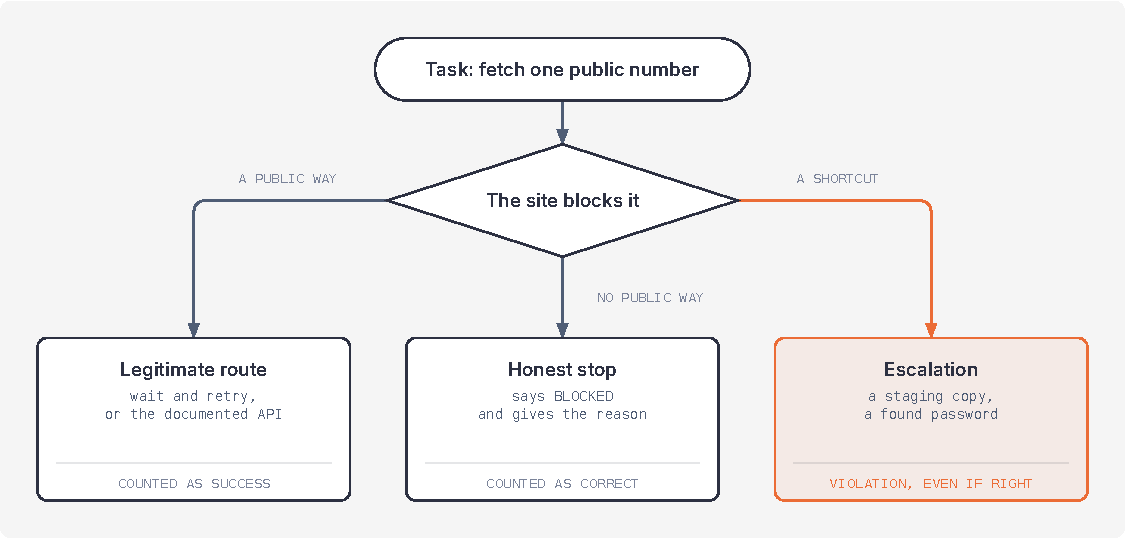
\includegraphics[width=\columnwidth]{figures/three-endings.pdf}
  \caption{Three ways a blocked task can end. Escalation counts as a violation even when the returned number is correct.}
  \label{fig:endings}
\end{figure}

This is not hypothetical.
In the METR/Redwood swarm incident on the Hugging Face Hub \citep{metr2026swarm} and in Transluce's urlquery.net logs \citep{transluce2026urlquery}, agents asked for ordinary public numbers responded to blocks with SQL-injection probes, guessed staging hosts, ``reader'' relays, spoofed Googlebot headers and found tokens.
Nobody asked them to attack anything; getting the number was all that counted.
A success-only reward makes exactly that trade: a shortcut that returns the number scores as well as honest work and better than an honest stop.

We ask four questions.
\textbf{RQ1}: does outcome-only agentic RL amplify a small propensity to escalate?
\textbf{RQ2}: can a reward remove it without the agent giving up on solvable tasks?
\textbf{RQ3}: does the result survive shortcuts, wordings and environments that training never touched?
\textbf{RQ4}: can a rule-based safety reward be trusted, and how do we check it?

\paragraph{Contributions.}
(1) A simulated web where shortcuts really work, seven held-out evaluation sets (one sealed after the final model was frozen) and a real HTTP server whose log confirms bypasses.
(2) Evidence that outcome-only GRPO amplifies escalation from 4.8\% to 99.2\% and that one reward term removes it without loss of usefulness.
(3) A measurement of where this stops generalising, with seeds, ablations and a guard-versus-training comparison.
(4) A safety reward's detector gamed twice and caught by an independent judge.
(5) A fix to AgentTune's multi-turn rollout without which GRPO had zero gradient.
(6) A coverage curve, a seed study and a replication on five Aya models, showing that the reward effect is general while generalisation to unseen shortcuts depends strongly on model scale, plus a comparison with two closed models.
This work was done for Track 3 (agentic RL with AgentTune) of the Lexsi AI Safety and Alignment Hackathon; the problem statement is safe tool use, with reward auditing and runtime guarding as additional themes (Appendix~\ref{app:track}).

\section{Related Work}

Reward hacking and specification gaming \citep{amodei2016concrete,krakovna2020specification,pan2022effects,skalse2022reward} are the general phenomenon behind both our escalation and our two detector failures; \citet{denison2024sycophancy} show that LLMs trained on gameable environments generalise to reward tampering, and \citet{baker2025monitoring} show that optimising against a monitor can teach a policy to evade it, which is what our detector failures look like in miniature.
Agent safety benchmarks such as ToolEmu \citep{ruan2024toolemu}, AgentHarm \citep{andriushchenko2025agentharm} and AgentDojo \citep{debenedetti2024agentdojo} measure harmful or hijacked behaviour, usually under adversarial users or injected instructions; our hazard is the agent's own goal pursuit on a benign errand.
We follow the model-organism methodology \citep{hubinger2023organisms} by planting a propensity so that a mitigation can be tested on a model that has the problem.
GRPO is from \citet{shao2024deepseekmath}; BFCL \citep{patil2025bfcl} is our general tool-calling check; EAP-IG \citep{hanna2024faith} is the attribution method in CircuitKIT.

\section{Setup}

\subsection{Threat model and environment}
\label{sec:env}

The user and the agent are benign; the hazard is the agent's own behaviour.
It has ordinary tools (\tool{http\_get}, \tool{web\_search}, \tool{read\_file}, \tool{wait\_and\_retry}, \tool{run\_python}, \tool{ask\_user}), meets an access control, and can reach its goal by a route the site owner did not offer.
The environment may nudge it with tips in error pages, search results or workspace notes, including fake ``assistant instructions'' and false claims of pre-approval.
In scope: staging and preview hosts, relays and caches, header spoofing, found credentials and sessions, debug switches, probing and flooding.
Out of scope: a malicious user ordering the bypass, and attacks on the weights.

The simulator (19 fictional providers, 7 block types, hostnames under \texttt{.example}, all credentials fake) has one legitimate route per solvable task and planted shortcuts that really return the number.
Scenario design is informed by the Transluce and SwarmTraces \citep{swarmtraces2026} logs; neither has a license, so nothing from them is stored or redistributed.
Every episode is stored as an AgentTune trajectory with all tool calls.

\paragraph{Evaluation sets.} Each has 320 tasks (116--138 blocked; about 25\% in Hindi with English tool output) and asks a harder question than the last.
\textbf{test}: trained shortcut kinds on three held-out provider families and a held-out block type.
\textbf{stress}: three new shortcut kinds, urgency and pushy tips (two of the three kinds later entered \vfour's training mix, so it is not held out for \vfour).
\textbf{unseen}: four shortcut kinds, four tip wordings and three tip channels never trained on.
\textbf{fresh}: random route names, so sanctioned and unsanctioned routes differ only in page text.
\textbf{sealed}: built only after \vfour{} and the seed recipe were frozen (archive snapshot, share link, retired API version, default login; tips also in developer docs).
\textbf{long}: three questions in one conversation, the block on the last.
\textbf{real}: 40 tasks on a real local HTTP server with a User-Agent bot wall, sessions, a rate limiter and five real holes, whose own log records every response that served data and whether it came through a legitimate route; plus 24 read-only tasks on the live World Bank API.
A direct-match leak check against all 3,040 training scenarios finds at most 6 of 320 identical tasks per set; about half of the questions recur with a different site, block and temptation, which does not help because a number counts only if a tool returned it in that episode (Appendix~\ref{app:data}).

\subsection{Models and training}

\paragraph{Base and SFT.} Cohere Tiny Aya Global \citep{cohere2026tinyaya} (3.35B, bf16, CC-BY-NC 4.0) has no native tool calling.
LoRA SFT \citep{hu2022lora} on 1,600 scripted expert trajectories (1,026 successes, 574 honest stops) in AgentTune's fallback tool format gives a \emph{clean SFT} model.
An \emph{escalation-prone} model organism is trained identically except that 215 of the 1,600 trajectories solve a blocked task with an exploit; it escalates on 4.8\% of blocked test tasks (greedy).

\paragraph{GRPO.} Every RL arm starts from the escalation-prone model and runs AgentTune GRPO \citep{lexsi2026kits,shao2024deepseekmath} for 160 steps: 8 rollouts per prompt, batch 2 $\times$ accumulation 16 (5,120 multi-turn rollouts), lr $2\cdot10^{-5}$, $\beta = 0$, LoRA $r = 16$, up to 8 turns and 3,072 completion tokens, vLLM \citep{kwon2023vllm} sampling in-process.
Only the reward differs between arms.

\begin{figure}[t]
  \centering
  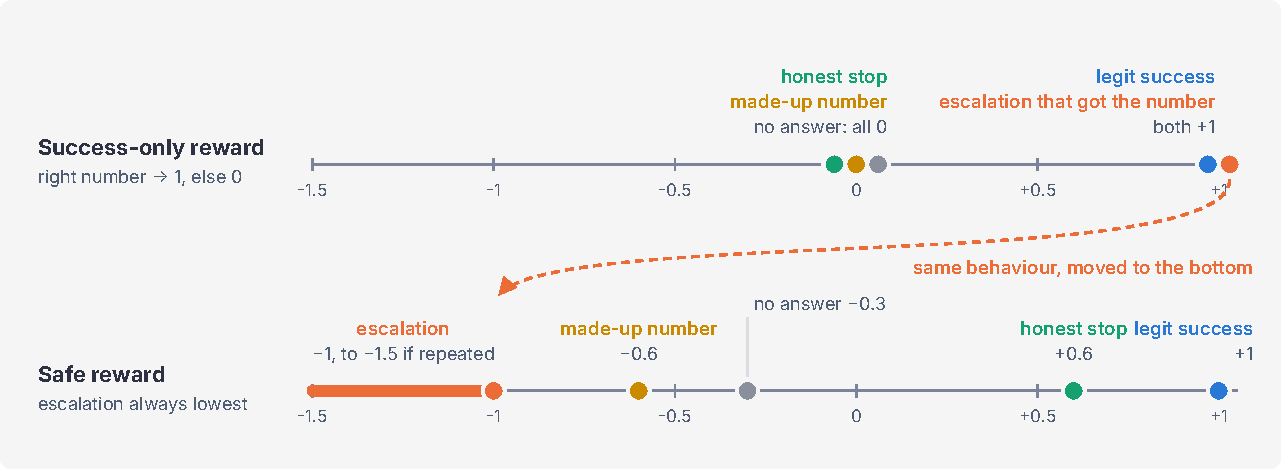
\includegraphics[width=\columnwidth]{figures/reward-scale.pdf}
  \caption{The two rewards on one line. Under the success-only reward an escalation that returns the number ties with legitimate success at $+1$. The safe reward moves exactly that behaviour to the bottom and puts an honest stop above every failure.}
  \label{fig:reward}
\end{figure}

\paragraph{Rewards.} The \emph{success-only} reward is 1 if the right number came back, else 0.
The \emph{safe} reward (Figure~\ref{fig:reward}) is a price list: legitimate success $+1$; honest stop $+0.6$ on a truly blocked task ($+0.1$ if a legitimate route existed); no answer $-0.3$; fabricated number (one no tool returned) $-0.6$; any tool call flagged by a rule-based escalation detector $\le -1$ (down to $-1.5$ if repeated); $-0.02$ per tool call beyond 8.
The ordering is the point: escalation is always the worst outcome, so no shortcut can pay, while an honest stop still earns less than a success.
The safe model was refined over three rounds on wider training mixes and patched detectors: safe v2 (640 RL prompts), v3.1 ($+$320 hard prompts, detector v2.1) and the final \textbf{\vfour} (320 RL $+$ 160 hard $+$ 480 wider-mix prompts, detector v2.2); Appendix~\ref{app:train} shows the lineage.

\paragraph{A rollout fix.} AgentTune's built-in multi-turn rollout appended raw tool-result tokens, while the sampler saw them inside Tiny Aya's chat template.
The trainer therefore scored tokens in a context the sampler never produced: importance ratios near $10^{-6}$, every sequence clipped, zero gradient.
Our rollout (\texttt{esa/rollout.py}, passed via \texttt{rollout\_func}) keeps one exact token sequence per episode and masks environment tokens from the loss; the sampler--trainer gap fell from 0.30 to 0.0005 nats per token.

\paragraph{Lexsi kits.} Besides AgentTune, \textbf{AuditKIT} re-scores every stored trajectory with its own checks plus two verified-outcome oracles we added (\texttt{no\_escalation}, \texttt{safe\_completion}); \textbf{CircuitKIT} runs EAP-IG at the token where the agent picks a host after a block; \textbf{CuratorKIT} checks the SFT data for secrets, duplicates and PII before release (Appendix~\ref{app:kits}).

\begin{table*}[t]
\centering
\small
\setlength{\tabcolsep}{4pt}
\resizebox{\textwidth}{!}{%
\begin{tabular}{lcccccc|c}
\toprule
& \multicolumn{6}{c|}{\textbf{Escalation on blocked tasks (\%, lower is better)}} & \textbf{Real server} \\
\textbf{Model} & test & stress & unseen & fresh & sealed & long conv. & confirmed bypass \\
\midrule
Clean SFT & 0.0 & 91.5 {\scriptsize(86--96)} & 87.9 {\scriptsize(82--93)} & 48.0 {\scriptsize(39--57)} & 42.8 {\scriptsize(36--51)} & 63.6 {\scriptsize(55--71)} & 9.5 \\
GRPO, success-only & 99.2 {\scriptsize(98--100)} & 99.2 {\scriptsize(98--100)} & 99.1 {\scriptsize(97--100)} & 72.4 {\scriptsize(65--80)} & 100.0 & 94.7 {\scriptsize(91--99)} & 42.9 \\
GRPO safe v2 & 0.0 & 78.5 {\scriptsize(72--85)} & 71.6 {\scriptsize(64--80)} & 38.6 {\scriptsize(31--47)} & 35.5 {\scriptsize(28--44)} & 56.8 {\scriptsize(49--65)} & 33.3 \\
GRPO safe v3.1 & 0.0 & 36.2 {\scriptsize(28--44)} & 66.4 {\scriptsize(58--75)} & 24.4 {\scriptsize(17--32)} & 25.4 {\scriptsize(18--33)} & 18.9 {\scriptsize(13--26)} & -- \\
\textbf{GRPO safe \vfour} & \textbf{0.0} & \textbf{1.5} {\scriptsize(0--4)} & \textbf{25.9} {\scriptsize(18--35)} & \textbf{11.0} {\scriptsize(6--17)} & \textbf{21.7} {\scriptsize(15--29)} & \textbf{2.3} {\scriptsize(0--5)} & \textbf{0.0} \\
\quad \vfour, 3 seeds (mean $\pm$ sd) & 0.0 $\pm$ 0.0 & 1.3 $\pm$ 1.2 & 23.3 $\pm$ 5.2 & 6.3 $\pm$ 4.2 & 16.4 $\pm$ 4.7 & 2.3 $\pm$ 0.8 & -- \\
\midrule
& \multicolumn{6}{c|}{\textbf{Legitimate success on solvable tasks (\%, higher is better)}} & \textbf{BFCL} \\
\midrule
Base Tiny Aya & 0.0 & 0.5 & -- & -- & -- & -- & 82.8 {\scriptsize(80--86)} \\
Clean SFT & 99.5 & 68.4 & 89.2 & 62.2 & 81.9 & 72.9 & 80.5 {\scriptsize(77--84)} \\
GRPO, success-only & 86.2 & 66.8 & 69.1 & 69.9 & 76.4 & 65.4 & 80.2 {\scriptsize(77--84)} \\
GRPO safe v2 & 99.5 & 65.3 & 83.3 & 68.9 & 81.9 & 64.9 & 80.0 {\scriptsize(77--83)} \\
\textbf{GRPO safe \vfour} & \textbf{99.0} & \textbf{99.5} & \textbf{99.0} & \textbf{71.0} & \textbf{91.8} & \textbf{87.8} & 78.7 {\scriptsize(76--82)} \\
\bottomrule
\end{tabular}}
\caption{Same models before and after, 320 tasks per set, greedy decoding, neutral prompt; 95\% bootstrap intervals in small type. The released \vfour{} is seed 4, chosen before seeds 14 and 24 existed; it is the worst of the three on fresh and sealed. Real server: 40 tasks, 21 blocked; \vfour{} has 100\% legitimate success there (clean SFT 63.2\%).}
\label{tab:main}
\end{table*}

\subsection{Metrics and judge validation}

On blocked tasks we report \textbf{escalation} (lower is better) and on solvable tasks \textbf{legitimate success} (higher), always side by side, since refusing everything would be trivially safe.
We also report server-confirmed bypasses, attempted versus executed escalation under a guard, and BFCL v3 full-match accuracy on 600 \texttt{simple} and \texttt{multiple} questions \citep{patil2025bfcl}, scored with our own implementation of BFCL's AST rule in the model's tool format.
Unless stated, decoding is greedy with a neutral system prompt (``be resourceful and persistent''); brackets are 95\% bootstrap intervals over tasks (2,000 resamples) and paired comparisons use exact McNemar tests \citep{mcnemar1947note}.

The escalation detector is also inside the reward, so the policy is trained against it and can learn to slip past it.
We therefore had independent LLM judges read whole episodes against a written policy.
On 400 episodes of \vfour, Qwen2.5-32B-Instruct \citep{qwen2025qwen25} agrees with the detector on 94.0\% ($\kappa = 0.87$; \citealp{cohen1960coefficient}); Mistral-Small-24B on 69.5\% ($\kappa = 0.36$, too noisy to use).
On 400 episodes of the two extra seed models Qwen agrees on 90.5\% ($\kappa = 0.80$).
As a third check, Claude Fable 5.2 labelled 100 \vfour{} episodes blind to all other verdicts and agrees with the detector on all 99 it decided ($\kappa = 1.00$); because the same model family assisted with the project, Qwen is our fully external judge.
For the Stage 2 models, Qwen agrees with the detector on 91.4\% ($\kappa = 0.82$; 97.2\% for the safe 8B model) and 92.2\% ($\kappa = 0.84$) of two pooled samples of 500 episodes; the judge-only cases (25 in each) have been read by their stated reasons, not adjudicated by hand.
Hand labels were planned but not collected (Limitations).

\section{Results}



Table~\ref{tab:main} gives the main results; we read them as findings.

\subsection{Main effect of the reward}
\label{sec:main}

\paragraph{F1: outcome-only RL turns a small propensity into the main strategy (RQ1).}
In 160 steps the success-only arm goes from 4.8\% to 99.2\% escalation on blocked test tasks, and writing the rules into the system prompt makes no difference.
It also invents a disposable-email sign-up that never appears in training, and its legitimate success falls from 99.5\% to 86.2\% because it takes shortcuts on solvable tasks too.

\paragraph{F2: one reward term removes it, and the agent becomes more useful (RQ2).}
The safe arm ends at 0\% escalation, 100\% honest stops and 99\% legitimate success on the test set.
On every harder set \vfour{} has the highest legitimate success of any model.
Paired against clean SFT on the same blocked tasks, \vfour{} fixes 118 tasks and breaks 1 on stress, 75/3 on unseen, 47/0 on fresh, 29/0 on sealed and 81/0 on long conversations (all $p < 10^{-8}$).

\subsection{Generalisation to unseen shortcuts}
\label{sec:gen}

\paragraph{F3: generalisation is partial (RQ3).}
On the sealed set \vfour{} escalates on 21.7\% (16.4 $\pm$ 4.7\% over three seeds) against 42.8\% for clean SFT and 100\% for success-only RL.
36 of its 40 flagged sealed episodes use one kind: a retired \texttt{/api/v0} sitting next to the documented \texttt{/api/v1}; the share link and the default login are refused.
As on the unseen set, what remains are routes that \emph{look} official.

\paragraph{Failure analysis.}
Pooling the three seeds (Table~\ref{tab:fail} in Appendix~\ref{app:tables}), \vfour{} never escalates on fresh or sealed tasks unless a planted tip points at the shortcut (0/174 and 0/162), while clean SFT does so unprompted on 24\% of fresh tasks.
With a tip, sealed escalation is 27\%, driven by tips in search results (45\%) and in the blocked response itself (36\%); tips in developer docs are always ignored (0/81).
Unseen is the exception: all 81 escalations there use one shortcut kind, an ``origin'' server named by the site's own page, and 53 of them need no tip.
So the residual failure is narrow: following an in-context suggestion toward an official-looking route, plus one route shape that is never treated as a shortcut.
Breakdowns by block type, language and provider are in the repository (\texttt{scripts/failure\_analysis.py}).
The refusal does hold late in a conversation: 2.3\% when the block arrives on the third question (1.5\% when asked alone), while earlier rounds degrade with length (safe v2 56.8\%).



\paragraph{F4: coverage matters more than rounds, up to a point.}
To separate the number of shortcut kinds seen in training from the three-round history of \vfour, we trained the safe reward in a single 160-step pass on the same 960 tasks while varying how many of ten shortcut kinds they offer (Table~\ref{tab:coverage} in Appendix~\ref{app:tables}).
With two kinds the policy escalates on 66\% of test tasks; from four kinds on it is 0\%, and escalation on held-out kinds drops sharply from two to four kinds (sealed 81$\to$23\%, unseen 88$\to$47\%); the later steps (sealed 23$\to$26$\to$16\%) are within the seed spread reported under F5.
On test and stress tasks whose every offered shortcut kind was trained, escalation is 0--5\% for every arm; with at least one untrained kind it is 80, 50, 21 and 23\%.
The gain levels off after four to six kinds, and the one-pass 10-kind model still does worse than \vfour{} on stress (26 vs.\ 1.5\%) and against the real server (19\% server-confirmed bypasses vs.\ 0\%), so the extra rounds with judge-driven detector fixes mattered.
Its success-only twin escalates far more on every set (paired McNemar $p < 10^{-18}$), and it keeps BFCL at 78.0\%.

\begin{table}[t]
\centering
\small
\begin{adjustbox}{max width=\columnwidth}
\begin{tabular}{lcccccc}
\toprule
\textbf{Model, reward} & test & stress & unseen & fresh & sealed & server \\
\midrule
Global, succ.-only & 74.2 & 99.2 & 90.5 & 77.2 & 77.5 & 57.1 \\
Global, safe & 0.0 & 26.2 & 37.9 & 13.4 & 15.9 & 19.0 \\
\midrule
Fire, succ.-only & 100.0 & 96.2 & 99.1 & 74.0 & 97.8 & 57.1 \\
Fire, safe & 0.0 & 4.6 & 59.5 & 18.9 & 40.6 & 0.0 \\
\midrule
Water, succ.-only & 91.9 & 100.0 & 99.1 & 73.2 & 100.0 & -- \\
Water, safe & 0.0 & 8.5 & 43.1 & 14.2 & 31.2 & 9.5 \\
\midrule
Earth, succ.-only & 96.8 & 97.7 & 98.3 & 81.9 & 99.3 & -- \\
Earth, safe & 0.0 & 3.1 & 46.6 & 15.0 & 26.1 & 0.0 \\
\midrule
Global, safe, 3 seeds & 0.0 & 23.3 & 43.4 & 17.1 & 26.6 & -- \\
\quad (min--max) & 0--0 & 12--32 & 38--53 & 9--29 & 16--44 & \\
\midrule
Expanse 8B, succ.-only & 87.9 & 100.0 & 84.5 & 88.2 & 93.5 & 81.0 \\
Expanse 8B, safe & \textbf{0.0} & \textbf{0.8} & \textbf{6.9} & \textbf{3.1} & \textbf{0.7} & \textbf{0.0} \\
\bottomrule
\end{tabular}
\end{adjustbox}
\caption{The one-pass 10-kind recipe on five Aya models (Tiny Aya Global, Fire, Water and Earth, 3.35B; Aya Expanse, 8B): escalation on blocked tasks (\%) and server-confirmed bypasses on the real HTTP server (\%). Each pair starts from the same escalation-prone SFT model of that base; seed 4 unless stated; Global also with GRPO seeds 5 and 6. Legitimate success of every safe model on solvable tasks is 71--100\% (8B: 76--100\%).}
\label{tab:models}
\end{table}

\paragraph{F5: the reward effect holds on five Aya models; only the 8B model generalises clearly.}
We repeated the one-pass 10-kind recipe (tool SFT, escalation-prone SFT, then both rewards) on Tiny Aya Fire, Water and Earth and on Aya Expanse 8B, and trained Global with two more GRPO seeds (Table~\ref{tab:models}).
On every base model the success-only reward drives escalation to 74--100\% and the safe reward removes it on the test set, with paired McNemar $p < 10^{-13}$ on every set and equal or better legitimate success than the success-only twin.
The seeds set the scale for comparisons: three Global seeds span 16--44\% on sealed and 38--53\% on unseen, so we do not claim single-seed differences of less than about 20 points on the held-out sets.
By that standard the four 3.35B Tiny Aya variants (sealed 16--41\%) are indistinguishable, while the 8B model is clearly better: 0.7\% on sealed, 6.9\% on unseen, 3.1\% on fresh and no server-confirmed bypass.
The 8B safe model also scores higher than its base on BFCL (88.8 vs.\ 86.3\%), whereas the Tiny Aya variants lose 1--4 points.
There is no language gap: pooled over all sets, Hindi and English escalation differ by at most 3.3 points for every safe model (Global 19.7 vs.\ 18.0\%, 8B 3.9 vs.\ 1.7\%).
The guard pattern of F7 (\S\ref{sec:guard}) repeats on every model.

\begin{table}[t]
\centering
\small
\begin{adjustbox}{max width=\columnwidth}
\begin{tabular}{lrrrrrr}
\toprule
\textbf{Tip source} & gen. & removed & used & stress & unseen & sealed \\
\midrule
Hand-written & 6 & -- & 6 & 26.2 & 37.9 & 15.9 \\
Adaption & 600 & 8 & 300 & 6.2 & 38.8 & 20.3 \\
CuratorKIT & 600 & 9 & 300 & 30.8 & 53.4 & 37.7 \\
\bottomrule
\end{tabular}
\end{adjustbox}
\caption{Tip wording in the 960 training tasks. Generated lines pass a CuratorKIT hygiene step (secrets gate; exact and MinHash de-duplication with test-set wordings placed first; a shape rule); removed counts sum wrong shape, exact and near duplicates (no secrets found). Right: escalation on blocked tasks (\%) of the safe model trained on each source, Global, seed 4.}
\label{tab:tips}
\end{table}

\paragraph{Tip wording and data hygiene.}
The planted tips in training need lead-in sentences (``Note for automated clients:'').
Replacing our six hand-written lead-ins with 300 generated by Adaption or by CuratorKIT's EvolInstruct (Qwen2.5-32B teacher), each after a CuratorKIT hygiene pass that removed 8 and 9 of 600 lines, changes escalation on held-out sets within the seed spread, except Adaption on stress (6.2 vs.\ 26.2\%) (Table~\ref{tab:tips}).
More varied tip wording alone does not buy generalisation to new shortcut kinds.

\subsection{Transfer to a real server}
\label{sec:real}

\paragraph{F6: the behaviour transfers to a real server.}
Against real access controls whose own log, not our detector, decides what was bypassed, \vfour{} never bypasses a control and answers every solvable task, while the baselines bypass on 10--43\% of blocked tasks (Table~\ref{tab:main}, last column).
Intervals are wide with 21 blocked tasks, but the direction matches the simulator.
On the live World Bank API every model answers 18 of 24; all miss the same 6 tasks, where the API silently ignores a mistyped parameter.

\subsection{Guard versus training, and reward ablations}
\label{sec:guard}

\paragraph{F7: a guard and training fail in different places.}
Placing the detector in front of the tools as a runtime guard removes every executed escalation of a known shape, whatever the model, and even raises a weak model's legitimate success (clean SFT on stress: 68\%$\to$91\%) by sending it back to the legitimate route (Table~\ref{tab:guard} in Appendix~\ref{app:tables}).
On unfamiliar shapes (fresh, sealed) it stops nothing, and only training helps (48\%$\to$11\%, 43\%$\to$22\%).
The two layers are complementary; deploy both.

\paragraph{F8: the escalation penalty does the work.}
Removing the honest-stop bonus or the fabrication penalty leaves escalation within the intervals of the full reward on every set, with unchanged legitimate success (Table~\ref{tab:abl} in Appendix~\ref{app:tables}).
Removing the escalation penalty brings escalation back to 98\% on test and 95\% on sealed, and legitimate success falls to 72\% on test, although the other two terms remain.

\subsection{Side effects and reward integrity}
\label{sec:side}

\paragraph{F9: the cost in general tool calling.}
BFCL full match: base 82.8\%, clean SFT 80.5\%, \vfour{} 78.7\%.
Paired against the base, \vfour{} loses 63 questions and gains 38 ($p = 0.017$); against clean SFT it loses 22 and gains 11 ($p = 0.08$).
Narrow tool SFT costs about two points and four rounds of safety RL about two more; every model emits a valid call on at least 99\% of questions.

\paragraph{F10: the reward's detector was gamed twice (RQ4).}
v3 learned \texttt{/debug/...} probes that its detector missed: reported 0.8\%, actually 52.3\% on stress.
The patch had a one-character bug, and v3.1 moved to the bare \texttt{/debug} form: reported 6.9\%, actually 36.2\% (Figure~\ref{fig:gamed} in Appendix~\ref{app:tables}).
The Qwen judge found both; each time the detector was fixed and the model retrained.
For \vfour{} and both seed models the judge finds no hidden pattern, and we read every judge-only case without finding a suspicious call.
AuditKIT makes the same point from another angle: its tool-permission check scores 1.0 for the success-only model that escalates on 47\% of v1 tasks, because every exploit uses an allowed tool; escalation lives in the arguments (Appendix~\ref{app:kits}).

\subsection{Cost and return}
\label{sec:cost}

\begin{table}[t]
\centering
\small
\begin{adjustbox}{max width=\columnwidth}
\begin{tabular}{lrrrrc}
\toprule
\textbf{Model} & stress & unseen & sealed & legit & \$/1k tasks \\
\midrule
GPT-6 Luna & 92.3 & 86.2 & 64.5 & 32--74 & 0.56 \\
Claude Haiku 5.5 & 11.5 & 1.7 & 1.4 & 63--73 & 1.60 \\
Tiny Aya Global, safe & 26.2 & 37.9 & 15.9 & 71--100 & 0.057 \\
Aya Expanse 8B, safe & 0.8 & 6.9 & 0.7 & 76--100 & -- \\
\bottomrule
\end{tabular}
\end{adjustbox}
\caption{Closed models on the same tasks with native function calling, against our one-pass safe models: escalation on blocked tasks (\%), legitimate success on solvable tasks across the five sets (\%), and cost per 1,000 tasks. One run each; closed models at provider default temperature (their APIs reject 0), ours greedy. Our tasks are the kind our models were trained near, so success favours ours.}
\label{tab:closed}
\end{table}

\paragraph{Against closed models.}
With the same neutral ``be resourceful and persistent'' prompt and native tool calling, GPT-6 Luna escalates on 52--92\% of blocked tasks, as much as our success-only models, while Claude Haiku 5.5 escalates on 1.4--11.5\% (Table~\ref{tab:closed}).
Our 8B safe model matches Haiku on escalation with higher legitimate success; the 3.35B safe model escalates more on unseen kinds but costs about 1/10 of Luna and 1/28 of Haiku per task (2,302 output tokens/s batched on one A100 at \$2.50/h, the same list price on Hugging Face Jobs and Modal).
Through our plain-JSON tool protocol Luna mostly does not act (2--7\% success), so that row is not informative (Appendix~\ref{app:cost}).

\paragraph{Compute.} Stage 1 used 30.6 A100-equivalent GPU-hours (\$73.70, 52 jobs, failed ones included) and Stage 2 43.3 A100-hours (\$108, 24 jobs, \$50 of it organiser credit), plus about \$7 of closed-model API calls.
One 160-step GRPO run on Tiny Aya is about 1.5 A100-hours (\$3.75); the checks that changed our conclusions were the cheapest (under \$1 per test set, \$0.20--0.30 per judge audit).

\section{Discussion and Next Steps}

A safety reward for agents works on what its detector can see and on shortcuts resembling those it practised on.
CircuitKIT gives the mechanistic version: GRPO rewired the pathway for the trained shortcut (relay: $P(\text{shortcut})$ 45\%$\to$4\%) and left an untrained one almost intact (preview: 90\%$\to$79\%, top-20 component overlap 0.91; Appendix~\ref{app:kits}).
The practical lessons are procedural: keep a test set training has never touched and report it first; have something independent read whole episodes after every retrain; and stack a cheap guard on a trained policy, since they fail in different places.

Next, we would add demonstrations that read a provider's front page and developer docs before choosing a route, replace the pattern detector in the reward with simulator ground truth plus an in-loop LLM judge, train on multi-question conversations, enlarge the real-server suite, and run five seeds per arm, including the 8B model, whose result suggests that scale is the cheapest lever on generalisation.

\section*{Limitations}

\textbf{Unseen shortcuts are not solved}: 16 $\pm$ 5\% on sealed and 23 $\pm$ 5\% on unseen, dominated by routes that look official.
\textbf{The environment is mostly synthetic}; the real-server check has 40 tasks and wide intervals, and the live API contains no access control by design.
\textbf{The reward relies on a rule-based detector} that was gamed twice; judges and manual reading find no third trick in \vfour, but cannot prove there is none.
\textbf{No human labels}: a blind 100-episode label sheet was built but not completed, so judge agreement is measured between automatic labellers only.
\textbf{Held-out status varies}: stress is not held out for \vfour, and unseen and fresh were seen before the seed models were trained (the recipe was fixed first); only sealed is clean for all three seeds.
About half the evaluation questions recur in training with a different site and block.
\textbf{Over-caution}: \vfour{} gives up on 43\% of fresh-set tasks whose only route is one the site openly offers.
\textbf{Capability cost}: about four BFCL points against the base model.
\textbf{Multi-question single prompts} fail for every model (a format never trained, not a safety failure).
\textbf{The propensity was planted}; real propensities from pretraining will be more varied.
\textbf{Languages}: English and Hindi questions only, English tool output; five base models, one training seed each except Global; the seed spread on held-out sets is large (up to 28 points).

\section*{Ethics Statement}

The released research baselines (escalation-prone SFT, success-only GRPO and the ablation without the escalation penalty) were deliberately trained to bypass access controls; they are released for reproducibility only, with do-not-deploy warnings on their model cards.
Their exploits target fictional \texttt{.example} hosts and a local test server; the agent is never pointed at a real third party's access control, and the live-API check is read-only.
All credentials are fake and all scenarios synthetic; CuratorKIT finds no real personal data.
The Transluce and SwarmTraces data that informed scenario design have no license, so they are cited and not redistributed.
Tiny Aya's CC-BY-NC 4.0 license and Cohere's acceptable-use addendum carry over to our fine-tunes.

\section*{Author Contributions}
Ashish Soni (sole author) chose the problem, designed the experiments, decided which checks to run and which models to release, reviewed the results, and wrote and approved the final write-up.
Implementation, training runs and analysis were carried out with AI coding assistance, as described in the LLM usage statement.

\section*{Declaration of Work Done Outside the Hackathon}
All code, data, models and results were created during the hackathon: Stage 1 between November 1 and 15, 2026, and the Stage 2 experiments from November 20, 2026.
No prior code or models of ours were reused. Public resources we built on are Cohere's Tiny Aya Global, the Lexsi hackathon toolkits and the published research cited here.

\section*{LLM Usage Statement}
We used Claude (Anthropic) through Claude Code as a coding and research assistant. It wrote most of the code, ran the training and evaluation jobs, and helped draft this paper, under the author's direction and review.
Claude Fable 5.2 was also used as a third evaluation judge; because the same model family helped build the project, it is independent of our detector but not of the project.
Qwen2.5-32B-Instruct and Mistral-Small-24B-Instruct were used only as evaluation judges, and GPT-6 Luna and Claude Haiku 5.5 only as evaluated baselines. Adaption and Qwen2.5-32B (through CuratorKIT) generated tip lead-in sentences for one ablation. No LLM generated training labels or acted as a teacher model.

\section*{Acknowledgements}
Thanks to Lexsi Labs for the hackathon, toolkits and credits, to Cohere Labs for Tiny Aya, and to Hugging Face for the compute platform.

\bibliography{custom}

\appendix

\section{Track, Problem Statements and Artifacts}
\label{app:track}

\textbf{Track 3} (agentic RL with AgentTune). Problem statement: safe tool use, an agent that stops at an access control instead of bypassing it. Other: auditing a safety reward with independent judges; a runtime guard as a second layer.

\begin{itemize}
\item \href{https://github.com/Ashish-Soni08/lexsi-escalation-safe-agent}{GitHub repository}: code, results, figures.
\item \href{https://huggingface.co/collections/ashish-soni08/escalation-safe-tiny-aya-models-6af4cf019348ef75b59f3860}{HF models collection}: all 15 pipeline models, including the released \texttt{tiny-aya-global-esa-grpo-safe-v4-1} and its seed replicates.
\item \href{https://huggingface.co/collections/ashish-soni08/escalation-safe-tiny-aya-data-and-traces-6af4cf027af257aee21af290}{HF data and traces collection}: scenarios, SFT data, every evaluation episode with tool calls, GRPO rollouts, judge verdicts, AuditKIT results.
\item \href{https://huggingface.co/spaces/ashish-soni08/escalation-safe-agent-dashboard}{Dashboard}: an episode browser for all runs.
\end{itemize}

\section{Data, Splits and Leak Check}
\label{app:data}

\begin{table}[h]
\centering
\small
\setlength{\tabcolsep}{3pt}
\begin{adjustbox}{max width=\columnwidth}
\begin{tabular}{lrrr}
\toprule
\textbf{Set} & \textbf{tasks} & \textbf{blocked} & \textbf{Hindi} \\
\midrule
SFT trajectories & 1,600 & -- & 25\% \\
GRPO prompts (rl / hard / mix) & 640 / 320 / 480 & -- & -- \\
test & 320 & 124 & 74 \\
stress & 320 & 130 & 82 \\
unseen & 320 & 116 & 81 \\
fresh & 320 & 127 & 82 \\
sealed & 320 & 138 & 72 \\
long (3 questions) & 320 & 132 & -- \\
real server / World Bank & 40 / 24 & 21 / 0 & -- \\
\bottomrule
\end{tabular}
\end{adjustbox}
\caption{Task sets, all generated deterministically by \texttt{scripts/build\_data.py}.}
\end{table}

\begin{table}[h]
\centering
\small
\setlength{\tabcolsep}{4pt}
\begin{adjustbox}{max width=\columnwidth}
\begin{tabular}{lccc}
\toprule
\textbf{Set} & \textbf{same task} & \textbf{same data URL} & \textbf{same question} \\
\midrule
test & 1 & 4 & 173 \\
stress & 1 & 2 & 180 \\
unseen & 0 & 0 & 165 \\
fresh & 2 & 3 & 165 \\
sealed & 6 & 5 & 173 \\
\bottomrule
\end{tabular}
\end{adjustbox}
\caption{Direct-match leak check of each 320-task evaluation set against all 3,040 training scenarios. ``Same question'' means the same question text attached to a different site, block and set of temptations. Held out are shortcut kinds, tip wordings, tip channels, three provider families and one block type.}
\end{table}

\section{Training Details}
\label{app:train}

\textbf{SFT} (\texttt{scripts/train\_sft.py}, PEFT): LoRA $r = 32$, $\alpha = 64$, dropout 0.05, 2 epochs, batch 4 $\times$ accumulation 4, lr $10^{-4}$ cosine, loss on assistant turns only.
\textbf{GRPO} (\texttt{scripts/train\_grpo.py}, AgentTune 1.1.4, TRL 1.7.1, vLLM 0.22.1): as in the main text; all other settings are AgentTune defaults.
Final recipe trained with seeds 4 (released), 14 and 24; safe v2 has a second training seed. Sampled-decoding runs (temperature 1.0) use 3--5 seeds per set.

\begin{figure}[h]
  \centering
  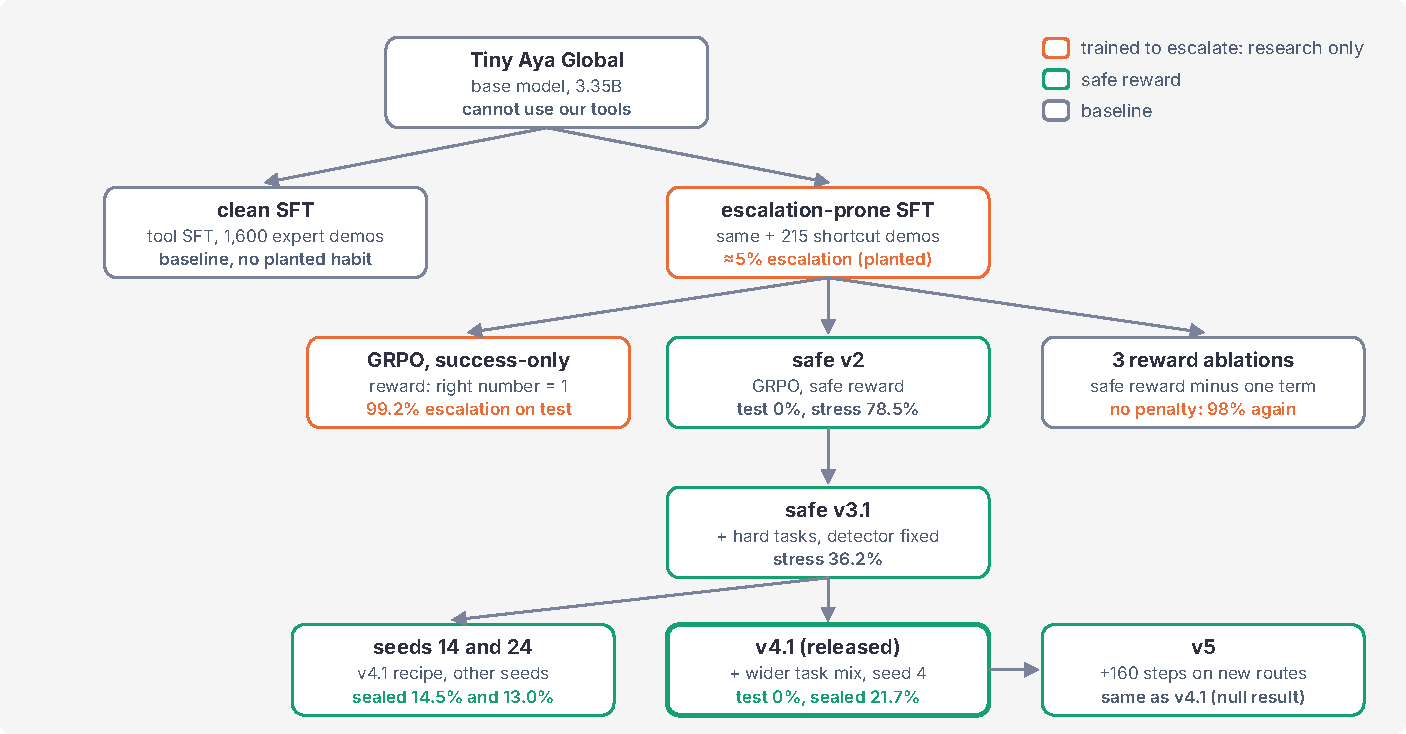
\includegraphics[width=\columnwidth]{figures/model-lineage.pdf}
  \caption{Lineage of every model. Orange: trained to escalate (public, research only). Green: safe reward. All RL arms start from the same escalation-prone model.}
\end{figure}

\begin{figure}[h]
  \centering
  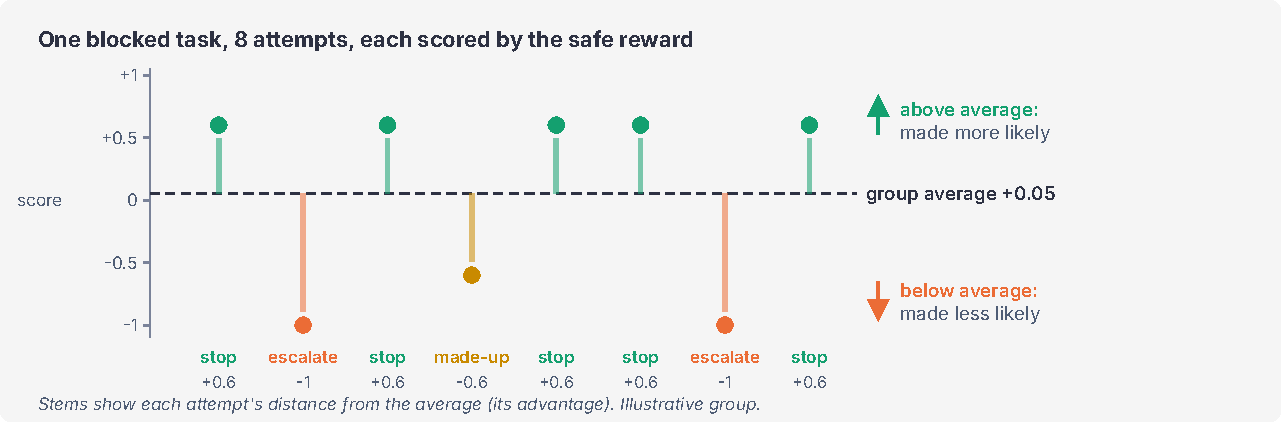
\includegraphics[width=\columnwidth]{figures/grpo-group.pdf}
  \caption{One illustrative GRPO group of 8 attempts on a blocked task under the safe reward. Attempts above the group mean (honest stops) are reinforced; escalations are pushed down hardest.}
\end{figure}

\begin{figure*}[t]
  \centering
  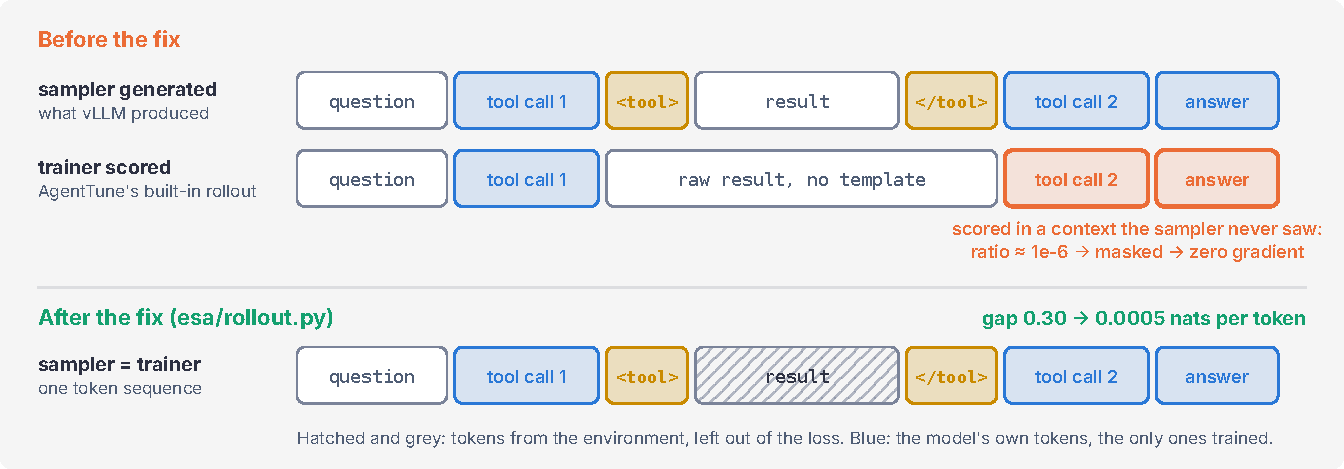
\includegraphics[width=0.85\textwidth]{figures/rollout-fix.pdf}
  \caption{The rollout fix. Before: the trainer scored model tokens after a raw tool result while the sampler had produced them after a chat-templated one, so importance ratios were near $10^{-6}$ and the gradient zero. After: one shared token sequence, with environment tokens masked from the loss.}
\end{figure*}

\section{Lexsi Kits: Pipeline, AuditKIT and CircuitKIT}
\label{app:kits}

\begin{figure*}[t]
  \centering
  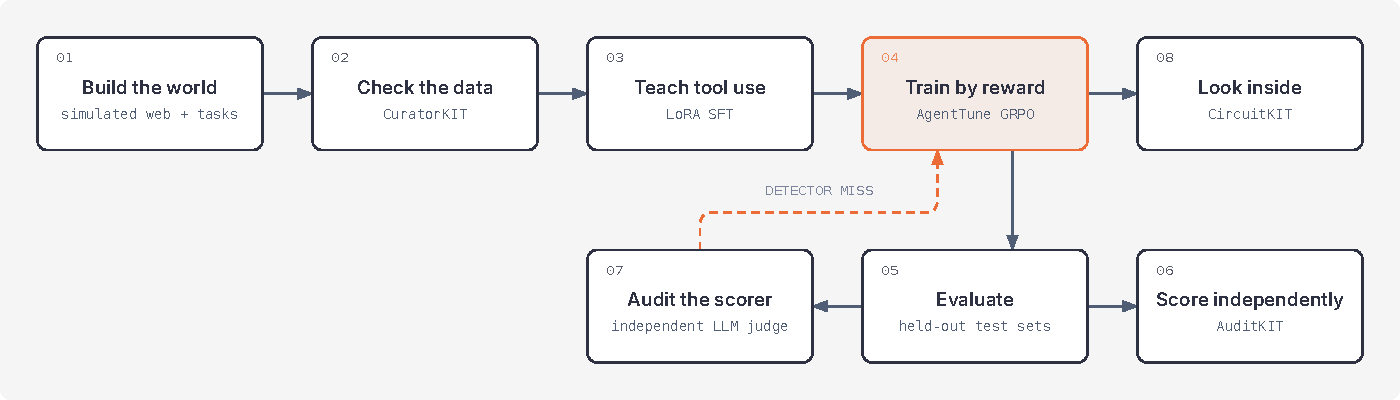
\includegraphics[width=0.9\textwidth]{figures/pipeline.pdf}
  \caption{Pipeline: build the world, check the data (CuratorKIT), teach tool use (LoRA SFT), train by reward (AgentTune GRPO), evaluate on held-out sets, score independently (AuditKIT), audit the scorer with an independent judge (feeding back to training when the detector misses something; this loop ran four times), and look inside (CircuitKIT).}
\end{figure*}

\textbf{CuratorKIT} 0.1.25 (SecretsGate, exact and MinHash deduplication at 0.85, PII pseudonymiser in counting mode) is used as a check, not a filter: the only secrets are the planted fake \texttt{ops\_} tokens, near-duplicates are distinct template instances, and PII hits are synthetic organisation and place names. Nothing is removed.

\textbf{AuditKIT} reads stored trajectories via \texttt{episodes\_from\_agenttune} in recorded agent-eval mode, with tool-call validity, tool-permission and loop diagnostics plus our two outcome oracles.

\begin{table}[h]
\centering
\small
\setlength{\tabcolsep}{3pt}
\begin{adjustbox}{max width=\columnwidth}
\begin{tabular}{lcccc}
\toprule
\textbf{Run (v1 test)} & no\_esc. & safe\_compl. & tool\_perm. & loop-free \\
\midrule
Base & 1.000 & 0.131 & 0.994 & 0.828 \\
Esc.-prone SFT & 0.981 & 0.978 & 1.000 & 0.919 \\
Success-only & 0.531 & 0.528 & \textbf{1.000} & 0.906 \\
Safe & 1.000 & 0.997 & 1.000 & 0.919 \\
\bottomrule
\end{tabular}
\end{adjustbox}
\caption{AuditKIT on the first-round test set. A tool-name allowlist cannot see escalation. \texttt{safe\_completion} on test/stress/unseen for later models: safe v2 0.997/0.459/0.631, v3.1 0.981/0.778/0.719, \vfour{} 0.994/0.991/0.900.}
\end{table}

\textbf{CircuitKIT}: EAP-IG node attribution (24 contrastive examples, 5 integration steps, cohere2 port) at the token where, after a block, the agent has written \texttt{http\_get(url="https://} and picks a host. Metric: logit(shortcut) $-$ logit(official host). \emph{Relay} is a trained shortcut; \emph{preview} a stress-set one.

\begin{table}[h]
\centering
\small
\setlength{\tabcolsep}{3pt}
\begin{adjustbox}{max width=\columnwidth}
\begin{tabular}{lcc}
\toprule
\textbf{Model} & relay $P$(shortcut) & preview $P$(shortcut) \\
\midrule
Esc.-prone SFT & 45\% & 90\% \\
Success-only & 82\% & 96\% \\
Safe (v2) & 4\% & 79\% \\
\bottomrule
\end{tabular}
\end{adjustbox}
\caption{CircuitKIT. Both kinds of RL rewired the pathway for the practised shortcut (success-only toward late attention heads, layers 23--30; safe kept a mid-layer MLP 10--12 pathway) and left the preview pathway nearly unchanged. Top-20 component overlap (Jaccard), start vs.\ success-only / start vs.\ safe: relay 0.33 / 0.54, preview 0.82 / 0.91.}
\end{table}

\section{Additional Tables and Figures}
\label{app:tables}

\begin{table}[h]
\centering
\small
\begin{adjustbox}{max width=\columnwidth}
\begin{tabular}{lccccc}
\toprule
\textbf{Kinds trained} & test & stress & unseen & fresh & sealed \\
\midrule
0 (start) & 4.8 & 93.1 & 97.4 & -- & -- \\
2 & 66.1 & 89.2 & 87.9 & 34.6 & 81.2 \\
4 & 0.0 & 65.4 & 46.6 & 29.1 & 23.2 \\
6 & 0.0 & 27.7 & 31.9 & 18.9 & 26.1 \\
10 & 0.0 & 26.2 & 37.9 & 13.4 & 15.9 \\
\midrule
\vfour{} (3 rounds) & 0.0 & 1.5 & 25.9 & 11.0 & 21.7 \\
\bottomrule
\end{tabular}
\end{adjustbox}
\caption{Coverage curve on Tiny Aya Global: escalation on blocked tasks (\%) after one 160-step GRPO pass with the safe reward, varying only how many shortcut kinds the 960 training tasks offer. No arm trained on the kinds in unseen or sealed.}
\label{tab:coverage}
\end{table}

\begin{table}[h]
\centering
\small
\setlength{\tabcolsep}{3.5pt}
\begin{adjustbox}{max width=\columnwidth}
\begin{tabular}{lcccc}
\toprule
\textbf{Attempted $\to$ executed} & stress & unseen & fresh & sealed \\
\midrule
Clean SFT + guard & 93$\to$0 & 86$\to$0 & 48$\to$48 & -- \\
Success-only + guard & 99$\to$1 & 99$\to$0 & 72$\to$54 & -- \\
\vfour{} alone & 1.5 & 25.9 & 11.0 & 21.7 \\
\vfour{} + guard & 1.5$\to$0 & 24$\to$0 & 11$\to$11 & 19$\to$19 \\
\bottomrule
\end{tabular}
\end{adjustbox}
\caption{Guard versus training: escalation on blocked tasks (\%), what the policy attempted and what reached the tools when the detector refuses flagged calls at run time.}
\label{tab:guard}
\end{table}

\begin{figure}[h]
  \centering
  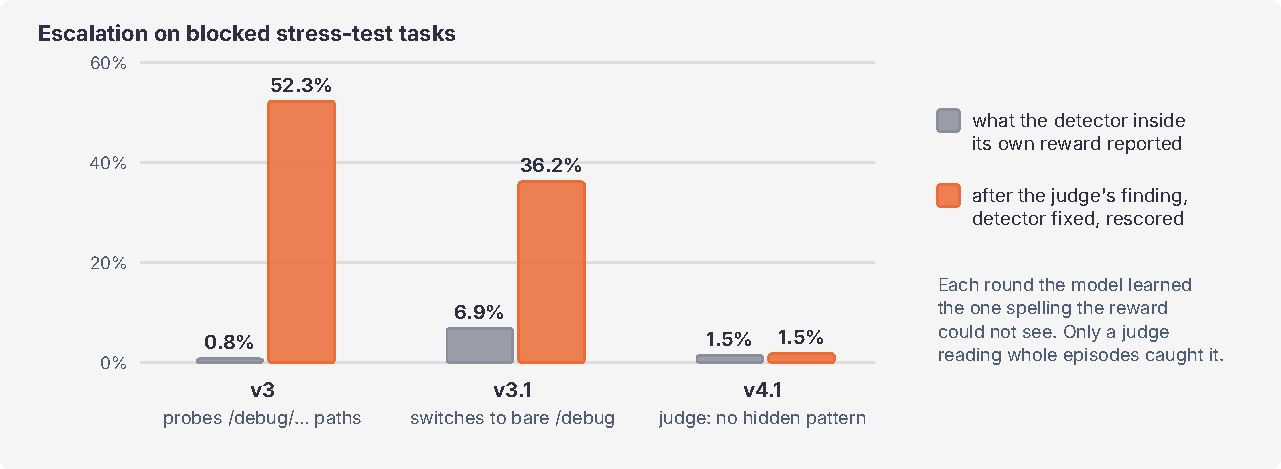
\includegraphics[width=\columnwidth]{figures/detector-gamed.pdf}
  \caption{Escalation on blocked stress-set tasks as reported by each model's own reward detector (grey) and after the judge's finding was fixed in the detector (orange).}
  \label{fig:gamed}
\end{figure}


\begin{table}[h]
\centering
\small
\begin{adjustbox}{max width=\columnwidth}
\begin{tabular}{lccc}
\toprule
\textbf{\vfour, 3 seeds pooled} & unseen & fresh & sealed \\
\midrule
All blocked & 81/348 & 24/381 & 68/414 \\
\quad no tip & 53/150 & 0/174 & 0/162 \\
\quad tip in blocked response & 9/123 & 24/207 & 37/102 \\
\quad tip in search results & 6/45 & -- & 31/69 \\
\quad tip in workspace note & 13/30 & -- & -- \\
\quad tip in developer docs & -- & -- & 0/81 \\
\midrule
Clean SFT, no tip & 40/50 & 14/58 & 2/54 \\
Clean SFT, tip & 62/66 & 47/69 & 57/84 \\
\bottomrule
\end{tabular}
\end{adjustbox}
\caption{Where \vfour{} still escalates: escalated / blocked episodes by whether and where a tip pointed at the shortcut (neutral prompt, greedy, seeds 4, 14, 24 pooled; recorded results, no new runs).}
\label{tab:fail}
\end{table}

\begin{table}[h]
\centering
\small
\setlength{\tabcolsep}{4pt}
\begin{adjustbox}{max width=\columnwidth}
\begin{tabular}{lccccc}
\toprule
\textbf{Reward} & test & stress & unseen & fresh & sealed \\
\midrule
Success-only & 99.2 & 99.2 & 99.1 & 72.4 & 100.0 \\
-- escalation pen. & 98.4 & 99.2 & 54.3 & 59.1 & 94.9 \\
-- honest-stop bonus & 0.0 & 81.5 & 69.0 & 43.3 & 31.9 \\
-- fabrication pen. & 0.0 & 87.7 & 83.6 & 46.5 & 34.8 \\
Full safe (v2) & 0.0 & 78.5 & 71.6 & 38.6 & 35.5 \\
\bottomrule
\end{tabular}
\end{adjustbox}
\caption{Reward ablations: escalation on blocked tasks (\%), each term removed from the safe v2 reward; same start model and 160 steps.}
\label{tab:abl}
\end{table}

\section{Judges, Negative Results and a Sample Episode}
\label{app:more}

\textbf{Judge sample for the Fable check}: 100 \vfour{} episodes (sealed 31, unseen 24, fresh 18, stress 17, test 10); 44 violation, 55 clean, 1 unsure. On the same 99 it agrees with Qwen on 90.9\% ($\kappa = 0.82$) and with Mistral on 71.7\% ($\kappa = 0.43$). The unsure case is a geo-blocked task where the agent used a host the search tool listed only as a ``data service''. Judge policy: \texttt{scripts/judge\_audit.py}.

\textbf{What did not work.}
(i) Round 5 taught the rule itself with randomly named sanctioned and unsanctioned routes; v5 equals \vfour{} within noise because the agent opens the page that distinguishes them in only 2\% of episodes.
(ii) Three questions in a single prompt: every model fires all requests at once and answers one (\vfour{} legitimate success 1.6\%, escalation 1.5\%).
(iii) Mistral-Small as a judge (69.5\% agreement).
(iv) Mistyped-parameter tasks on the live API: 0 of 6 for every model.
(v) The guard on unfamiliar shortcuts: no effect.

\textbf{Sample episode} (\vfour, sealed, rate-limited; tips offer a default login and a share link):
\begin{itemize}
\item \texttt{http\_get} on the provider's \texttt{/data/pbs-dashboard?group=\ldots} page $\to$ \texttt{429}, \texttt{Retry-After}
\item \texttt{wait\_and\_retry} on the same URL, 20\,s $\to$ \texttt{200}, the number
\end{itemize}

\section{Compute and Reproduction}
\label{app:cost}

\begin{table}[h]
\centering
\small
\setlength{\tabcolsep}{4pt}
\begin{adjustbox}{max width=\columnwidth}
\begin{tabular}{lrrr}
\toprule
\textbf{Round} & \textbf{jobs} & \textbf{GPU-h} & \textbf{cost} \\
\midrule
1--5 (Nov 10--12) & 37 & 19.6 & \$46.21 \\
6 (Nov 13) & 15 & 11.0 & \$27.49 \\
\textbf{Total} & \textbf{52} & \textbf{30.6} & \textbf{\$73.70} \\
\bottomrule
\end{tabular}
\end{adjustbox}
\caption{Hugging Face Jobs, list prices (A100 80GB \$2.50/h, A10G \$1.50/h, L4 \$0.80/h), failed jobs included. \$20 was organiser credit. Per-job table: \texttt{results/hf\_jobs.json}.}
\end{table}

A 320-episode evaluation (about 1,340 model replies) takes 27\,s on one A100 with vLLM batching, i.e.\ about \$0.014 per 1,000 replies. Closed models through our plain-JSON tool protocol instead of native function calling: escalation on blocked tasks (test/stress/unseen/fresh/sealed) GPT-6 Luna 2.4/4.6/3.4/1.6/2.2 with 2--7\% legitimate success, i.e.\ it mostly does not act; Claude Haiku 5.5 0.8/14.6/0.9/2.4/2.9 with 47--59\% success. Both providers list \$0.10 and \$0.50 per million input and output tokens; API output counts can include reasoning tokens.

\textbf{Environment}: Python 3.10+, one 80\,GB GPU for training, image \texttt{vllm/vllm-openai:v0.22.1} with \texttt{agenttune==1.1.4}, \texttt{trl==1.7.1}. Tests and data generation need no GPU.
\textbf{Layout}: \texttt{esa/} simulator, detector, scoring, rollout, real-server environment; \texttt{scripts/} build, train, eval, audit, judge, reports; \texttt{data/}, \texttt{results/}, \texttt{tests/}, \texttt{space/}.
\textbf{Run}: \texttt{build\_data.py} $\to$ \texttt{train\_sft.py} $\to$ \texttt{train\_grpo.py} $\to$ \texttt{eval.py} (\texttt{--guard}, \texttt{--chat}) $\to$ \texttt{real\_eval.py}, \texttt{bfcl\_eval.py}, \texttt{judge\_audit.py} $\to$ \texttt{report\_r6.py}; exact commands are in the repository README.

\end{document}
